\begin{frame}{Hyperparameter Sensitivity}

Let $\t$ be some real-valued hyperparameter for the stick-breaking density.
%(For example, $\t$ could be $\alpha$, or parameterize a functional shape).  
\pause

Write $\etaopt(\t) := \argmin_{\eta} \KL{\eta, \t} = \argmin_{\eta} \KL{\q(\zeta \vert \eta) || \p(\zeta \vert \x, \t)}$.
\pause

{\bf Problem:} Evaluating $\etaopt(\t)$ requires solving a new optimization problem.
\pause

%\pause

{\bf We propose: } Approximate $\etaopt(\t)$ with a first-order
Taylor expansion:

\begin{align*}
  \etaopt(\t)  &\approx  
  %\etalin(\t) := 
  \etaopt(0) + \fracat{d \etaopt(\t)}{d \t}{\t=0} \t. 
\end{align*}
%
\pause
%
\vspace{-0.5em}
\begin{itemize}
\item<5-> We need only use a linear approximation for the map $\t \mapsto \etaopt(\t)$. We can retain nonlinearities in the map 
$\etaopt \mapsto \expect{\q(\zeta \vert \etaopt)}{\#\text{clusters}}
$, etc.
\vspace{0.5em}
\item<6-> This is ``Bayesian local robustness'' for VB \citep[cf.][]{gustafson:1996:local}
\vspace{0.5em}
\item<7-> The derivative can be evaluated using the implicit function theorem
and modern
{\color{blue} \href{https://jax.readthedocs.io/en/latest/}{automatic differentiation}}.
\end{itemize}
\end{frame}







\begin{frame}{Computing the Derivative \citep{giordano:2018:covariances}}

\textbf{Theorem 1.} (The derivative $d\etaopt(\t) / d\t$.)  

\onslide<2-> {
Define $\etaopt = \etaopt(0)$, $\hessopt := \fracat{\partial^2 \KL{\eta}}
                {\partial \eta \partial \eta^T}
                {\etaopt}$ and 
$\lqgrad{\nu \vert \etaopt} :=
    \fracat{\log \q(\nu \vert \etaopt)}{\partial \eta}{\etaopt}$.
}

\onslide<3->Assume:
\begin{itemize}
    \item<3-> The Hessian at the optimum, $\hessopt$, is non-singular. %\pause
    \item<4-> The optimal VB parameters, $\etaopt$, are interior. %\pause
    \item<5-> We can exchange limits and $\q$ expectations as needed in a 
        neighborhood of $\etaopt$ and $\t=0$.  %\pause
    \begin{itemize}
        %\item Dominated convergence theorem on a laundry list of functions.
        \item This imposes some regularity conditions on the prior $\p(\nu \vert \t)$.
    \end{itemize}
\end{itemize}

\onslide<6->{
Then the map $\t \mapsto \etaopt(\t)$ is continuously
differentiable at $\t=0$ with
%
\begin{align*}
%
\fracat{d \etaopt(\t)}{d \t}{0} ={}&
    - \hessopt^{-1}
    \expect{\q_{\etaopt}}{
        \lqgrad{\nu \vert \etaopt}
        \fracat{\partial \log \p(\nu \vert \t)}{\partial \t}{\t=0}
    }.
%
\end{align*} \hfill $\square$
}

\onslide<7->{
{\bf Note:} The computation of $\hessopt^{-1}$ is the computationally 
difficult part.  For our BNP problem, $\hessopt$ is sparse.
}

\end{frame}

\begin{frame}{A Simple Example: Iris Data}

We fit a Gaussian mixture model with a DP prior to
the iris data.

\begin{figure}[!h]
  \centering
  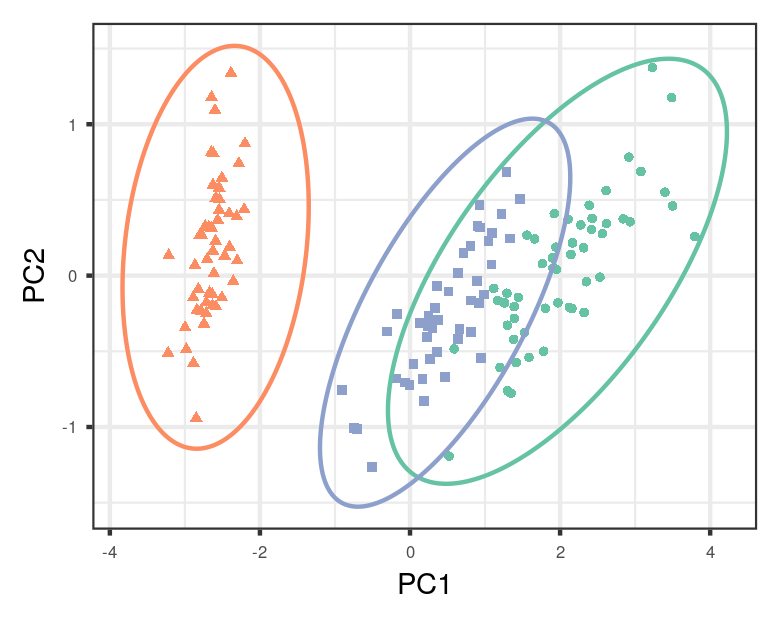
\includegraphics[width = 0.6\textwidth]{./figure/iris_init-1.png}
  \caption*{The iris data in principal component space and GMM fit at $\alpha = 6$.}
\end{figure}

\end{frame}

\begin{frame}{Iris Data: Parametric Sensitivity}

\begin{figure}[!h]
  \only<1>{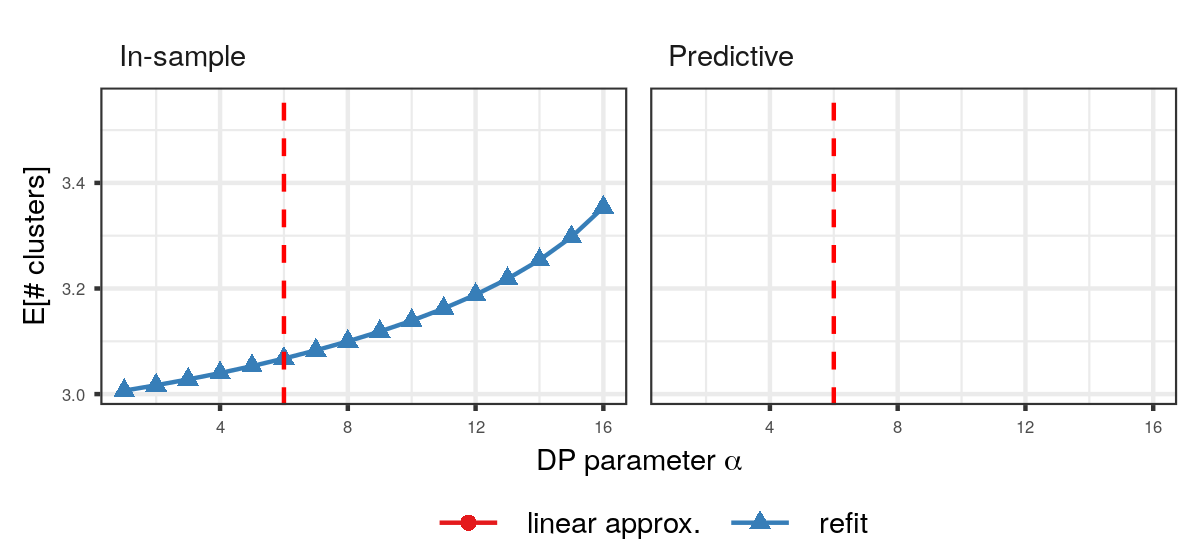
\includegraphics[width = \textwidth]{./figure/iris_alphasens_refit-1.png}}%
  \only<2>{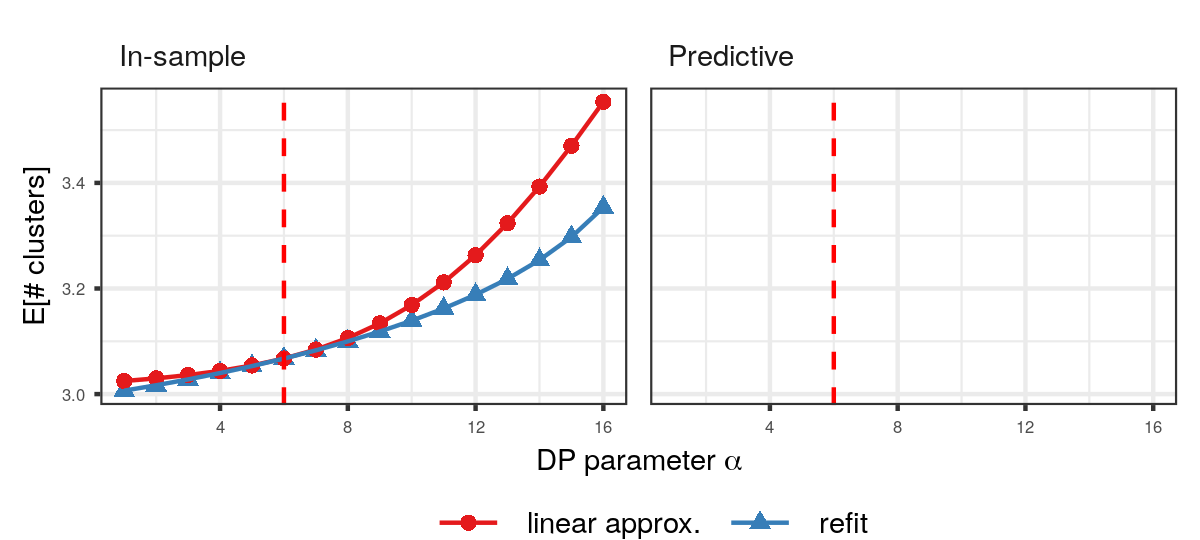
\includegraphics[width = \textwidth]{./figure/iris_alphasens_insample-1.png}}%
  \only<3>{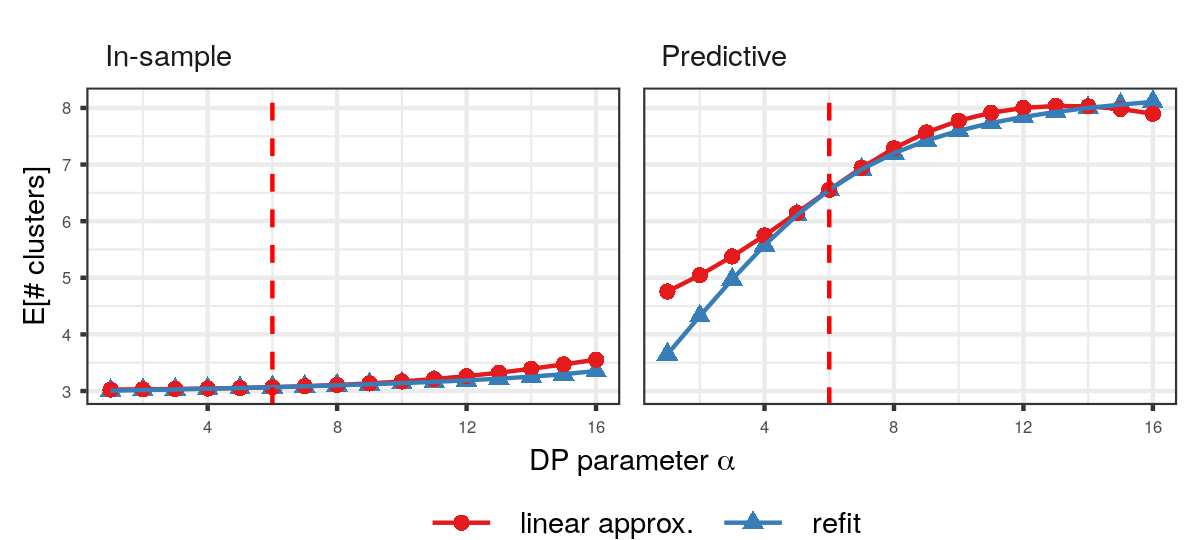
\includegraphics[width = \textwidth]{./figure/iris_alphasens_all-1.png}}
  \caption*{The expected number of posterior clusters in the iris data as $\alpha$ varies.}
\end{figure}

\end{frame}
